\documentclass[titlepage]{jarticle}
\usepackage[dvipdfmx]{graphicx}
\usepackage{here}
\begin{document}
 \part*{体育祭追加資料}
 体育祭企画書において、一部競技に関する図が分かりにくいため、補足するための資料である。\\
 また、明示されてない限り図下側を本部側とする。\\
同時に配った体育祭メンバー用紙は特に回収しませんので、各自で管理すること。また、リレーはアンカーを担当する団長を含めず2人用意すること。
 \section{リレー競技図}
  スタート、及びゴールの明記。
   \begin{figure}[H]
    \centering
    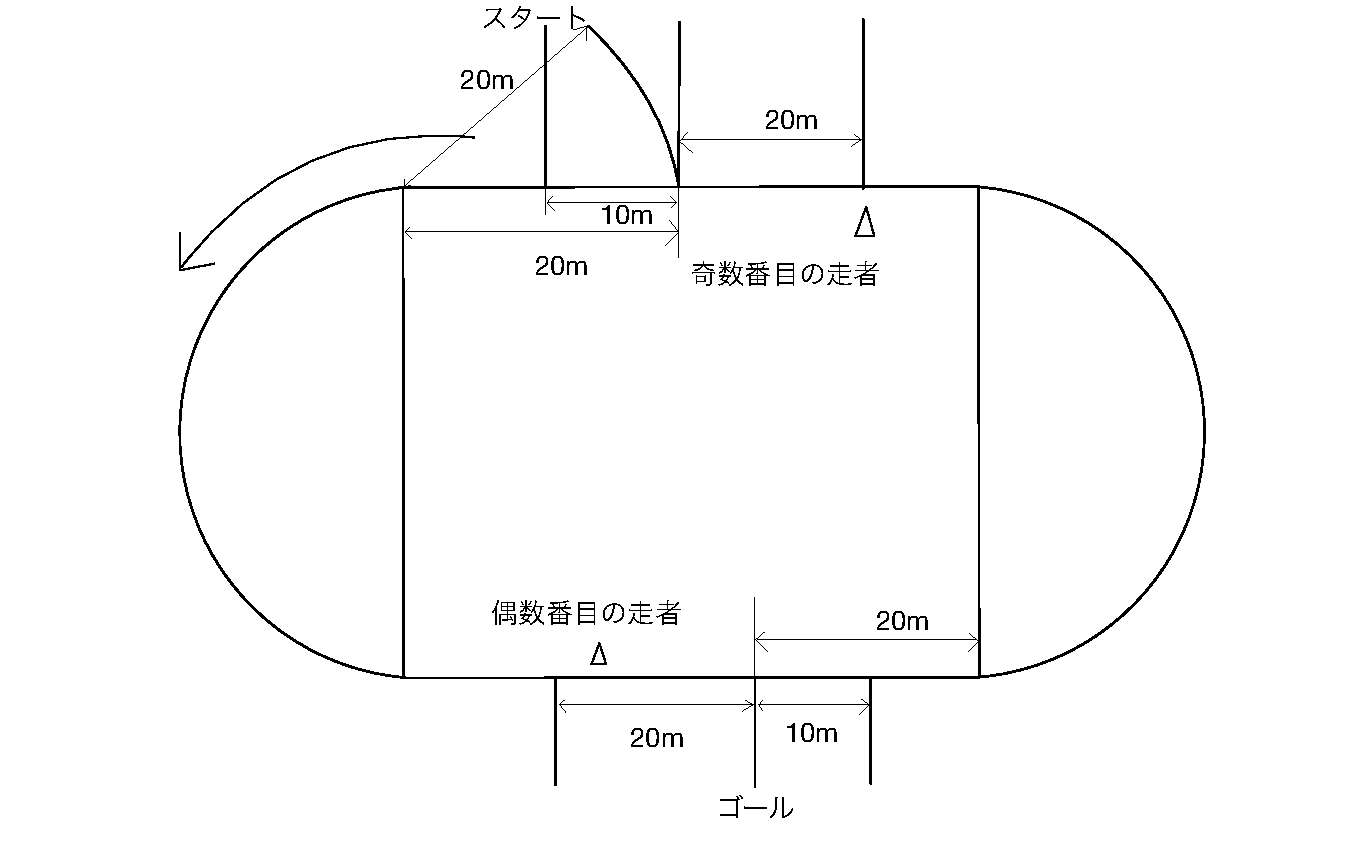
\includegraphics[width=12cm]{rire3.pdf}
    \caption{リレー競技図}
   \end{figure}
 \section{体育倉庫周辺}
  体育倉庫の場所がわからない人がいることが考えられるため。
 \begin{figure}[H]
    \centering
    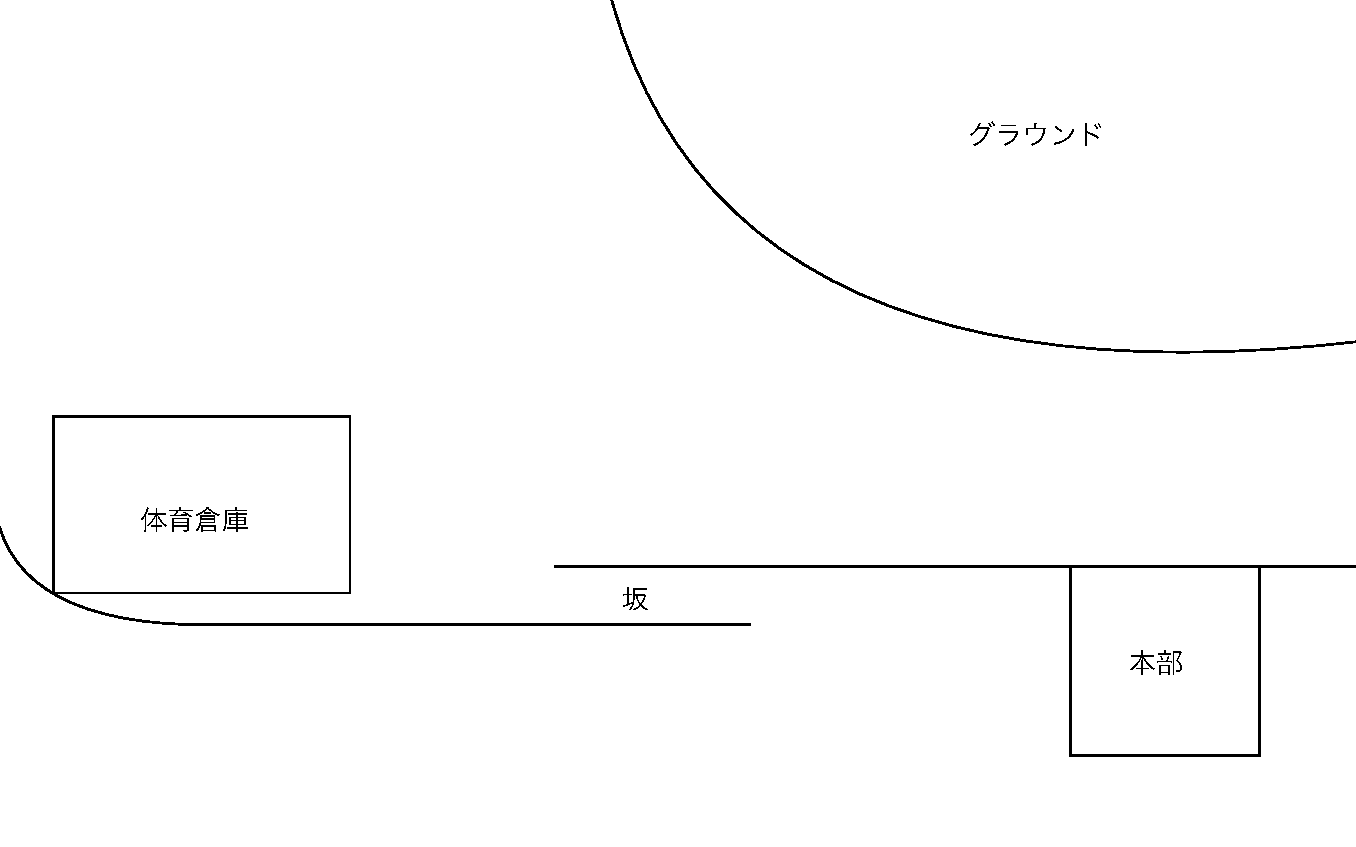
\includegraphics[width=12cm]{syugo.pdf}
    \caption{集合場所}
   \end{figure}
 \section{体育祭競技用ライン}
   \begin{figure}[H]
    \centering
    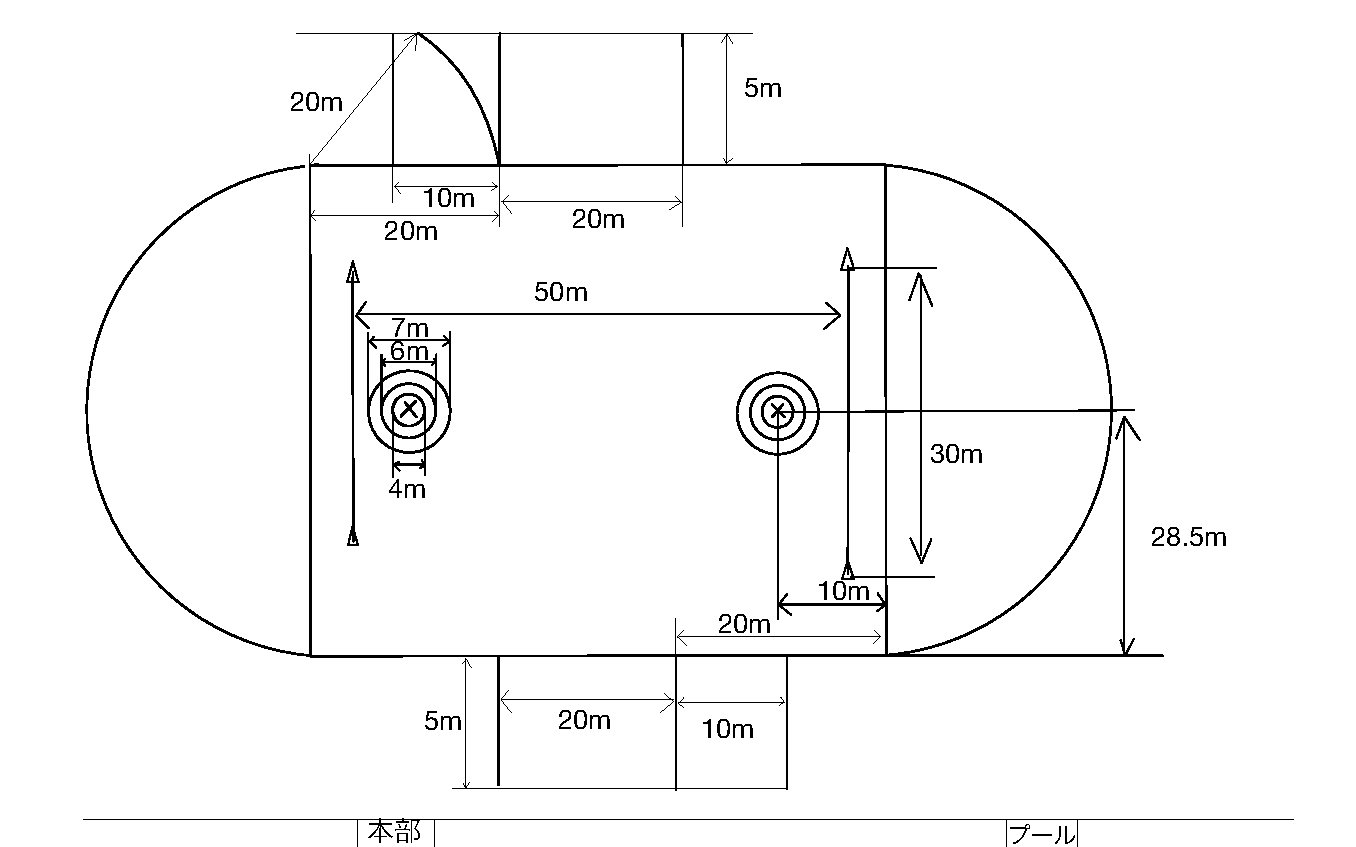
\includegraphics[width=12cm]{line.pdf}
    \caption{競技用ラインまとめ}
   \end{figure}
\end{document}